\section{Results}
\subsection{Two body system}
\begin{figure}[h]
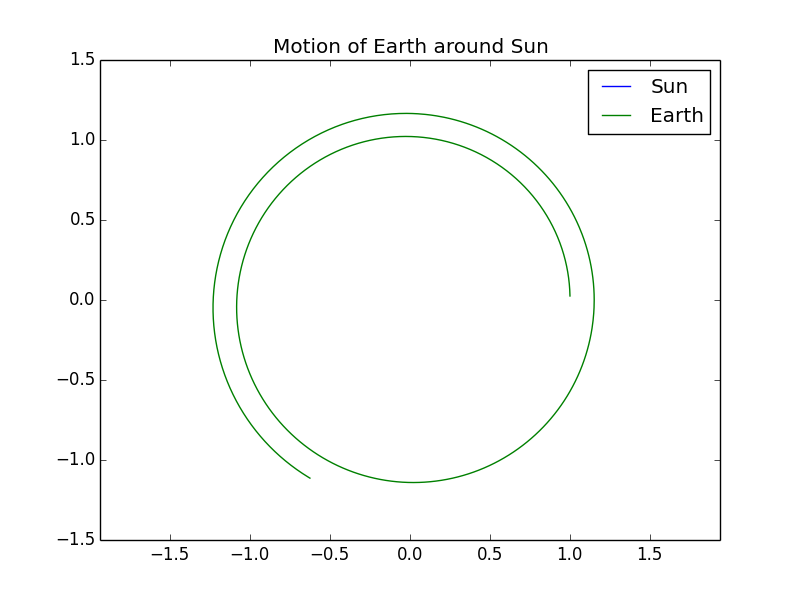
\includegraphics[scale=0.7]{figures/earth_sun_euler}
\caption{The plot shows the simulated orbit of the Earth around the Sun using the forward Euler integration method. The motion is simulated for two years, with $\Delta t = 0.002$ years.}
\end{figure}


\begin{figure}[h]
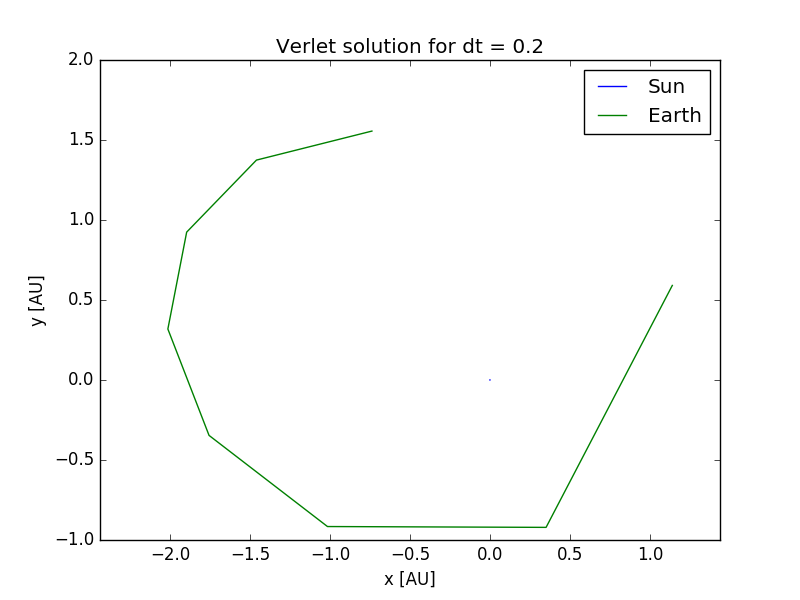
\includegraphics[scale=0.7]{figures/verlet_02}
\caption{The plot shows the simulated orbit of the Earth around the Sun using the velocity-Verlet integration method. The motion is simulated for two years, with $\Delta t = 0.2$ years}
\end{figure}

\begin{figure}[h]
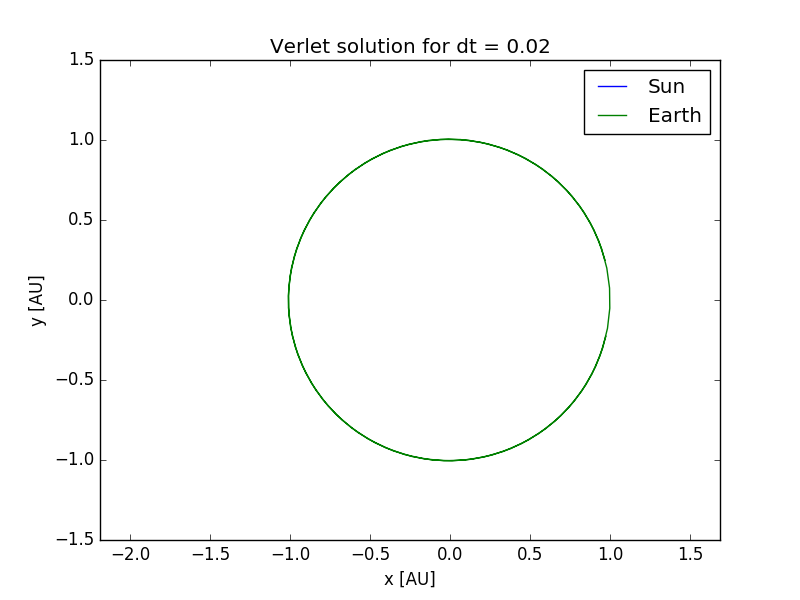
\includegraphics[scale=0.7]{figures/verlet_002}
\caption{The plot shows the simulated orbit of the Earth around the Sun using the velocity-Verlet integration method. The motion is simulated for two years, with $\Delta t = 0.02$ years}
\end{figure}



\begin{figure}[h]
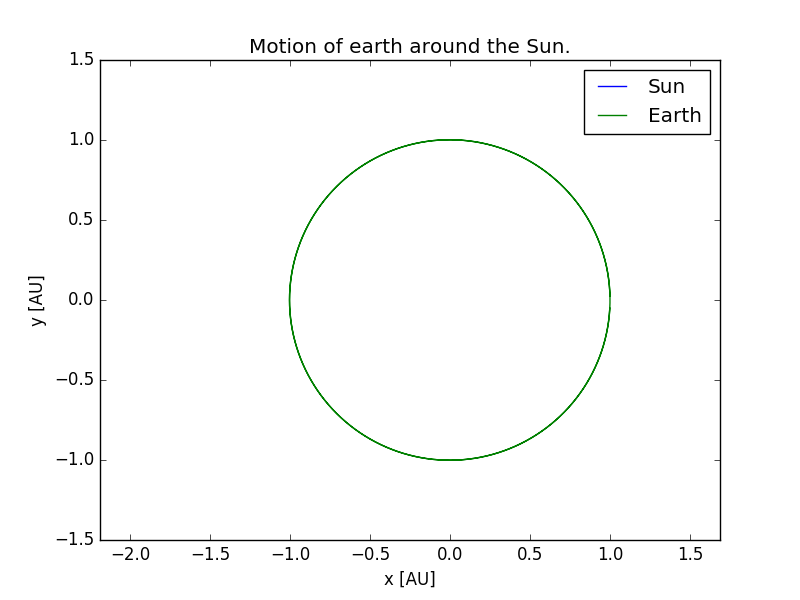
\includegraphics[scale=0.7]{figures/earth_sun_verlet}
\caption{The plot shows the simulated orbit of the Earth around the Sun using the velocity-Verlet integration method. The motion is simulated for two years, with $\Delta t = 0.002$ years.}
\end{figure}

The Euler method does not pass the tests for conservation of kinetic energy, potential energy and angular momentum for $\Delta t = 0.002$\ref{•}


\subsection{Three body system}
\begin{figure}[h]
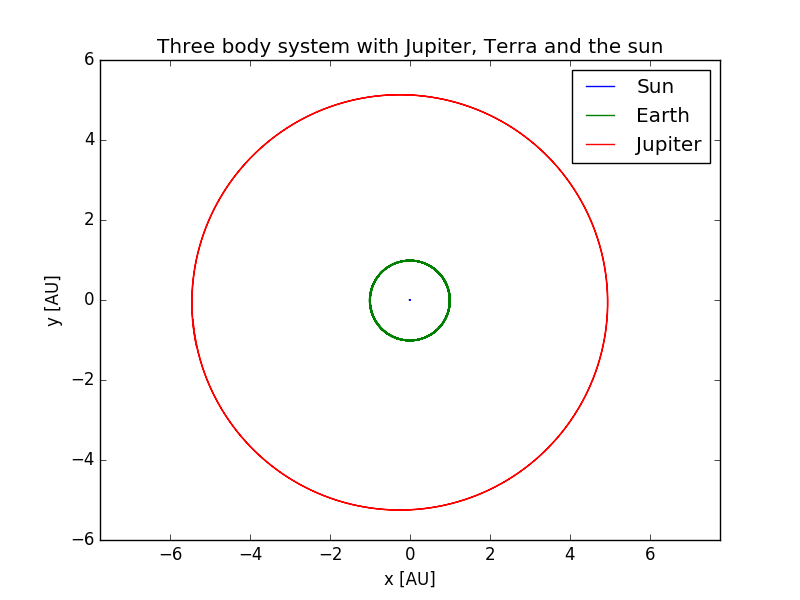
\includegraphics[scale=0.7]{figures/three_body}[h]
\caption{The plot shows the orbit of Earth and Jupiter around the Sun }
\end{figure}


